\documentclass[a4paper,11pt]{article}
  
\usepackage{graphicx}
\usepackage{amsmath}
\usepackage{array}
\usepackage{float}
\usepackage{subfigure}
\usepackage{color}
\usepackage{listings}
\usepackage[utf8x]{inputenc}
\usepackage[colorlinks=true,linkcolor=red,citecolor=blue]{hyperref}
\usepackage{rotating}
\usepackage{cite}
\usepackage{enumitem}

\usepackage{amsfonts,amsmath,amsthm,amssymb}
\usepackage{algorithm}
\usepackage{algpseudocode}

\renewcommand{\algorithmicrequire}{\textbf{Input:}}
\renewcommand{\algorithmicensure}{\textbf{Output:}}

%% --------- Algorithms -------------
\providecommand{\BeginAlgSize}[0]{\begin{scriptsize}}
\providecommand{\EndAlgSize}[0]{\end{scriptsize}}
\providecommand{\ForEach}[1]{\For{\textbf{each} #1}}
\providecommand{\Or}[0]{O}
\providecommand{\A}[0]{\mathbf{\alpha}}
%% --------- End of Algorithms -------------



% Read MRPT version:
\newread\file
\openin\file=../../version_prefix.txt
\read\file to\MRPTVERSION % Reads a line of the file 
\closein\file

% Title Page
\title{User guide for \texttt{libmrpt-srba}: A generic C++ framework for Relative Bundle Adjustment (RBA)}
\author{Jose-Luis Blanco-Claraco \\ joseluisblancoc@gmail.com \\ \texttt{http://www.mrpt.org/} }
\date{MRPT version: \MRPTVERSION \\ Document build: \today }

% C++ listings settings
\lstset{ %
language=C++,                % choose the language of the code
basicstyle=\scriptsize,       % the size of the fonts that are used for the code
numbers=none,                   % where to put the line-numbers
numberstyle=\footnotesize,      % the size of the fonts that are used for the line-numbers
stepnumber=1,                   % the step between two line-numbers. If it is 1 each line will be numbered
numbersep=5pt,                  % how far the line-numbers are from the code
backgroundcolor=\color{white},  % choose the background color. You must add \usepackage{color}
commentstyle=\color{blue},
showspaces=false,               % show spaces adding particular underscores
showstringspaces=false,         % underline spaces within strings
showtabs=false,                 % show tabs within strings adding particular underscores
frame=single,           % adds a frame around the code
tabsize=2,          % sets default tabsize to 2 spaces
captionpos=b,           % sets the caption-position to bottom
breaklines=true,        % sets automatic line breaking
breakatwhitespace=false,    % sets if automatic breaks should only happen at whitespace
escapeinside={\%*}{*)}          % if you want to add a comment within your code
}

\begin{document}
\maketitle


\vfill

\begin{scriptsize}
\begin{center}

\includegraphics[width=3cm]{imgs/by-nc-nd-eu.pdf}
\\
This work is licensed under a Creative Commons Attribution-NonCommercial-NoDerivs 3.0 Unported License.
\end{center}
\end{scriptsize}

\vspace{1cm}

\newpage

\textbf{Revision history:}
\begin{itemize}
 \item May 2013: Second version. Added Fig.~\ref{fig:Nr} and the section on spanning trees.
 \item March 2013: First version. Released along MRPT 1.0.0.
\end{itemize}

\vfill


\begin{small}
In case you want to cite SRBA in your academic publications, here is a BibTeX entry: 

\begin{verbatim}
@INPROCEEDINGS{blanco2013srba,
  author = {Blanco, J.L. and Gonzalez-Jimenez, J. and Fernandez-Madrigal, J.A.},
  month = {{may}},
  title = {{Sparser Relative Bundle Adjustment (SRBA): constant-time 
    maintenance  and local optimization of arbitrarily large maps}},
  booktitle = {IEEE International Conference on Robotics and Automation (ICRA)},
  year = {2013}
}
\end{verbatim} 

\noindent and here the one for this guide:

\begin{verbatim}
@MISC{libmrpt-srba-guide,
  author = {Jose-Luis Blanco-Claraco},
  title = {{User guide for \texttt{libmrpt-srba}: A generic 
      C++ framework for Relative Bundle Adjustment (RBA)}},
  howpublished = {http://www.mrpt.org/srba},
  year = {2013}
} 
\end{verbatim} 

\end{small}

\vspace{1cm}

\newpage
\tableofcontents
\newpage

\section{Introduction}

Bundle adjustment (BA) is the name given to one solution to visual Simultaneous Localization and Mapping (SLAM) (or Structure From Motion, SFM) 
based on maximum-likelihood estimation (MLE) over the space of map features and camera poses. 
However, it is by no way limited to visual maps, since the same 
optimization techniques employed in BA are also applicable to many other 
kind of feature maps, not necessarily involving visual information, or even to maps of pose constraints 
(\emph{Graph-SLAM}).

For readers without a solid background in mobile robotics or computer vision, it is \emph{strongly} recommended 
to start reading seminar works on SLAM \cite{thrun2005pr,durrantwhyte2006sla,bailey2006sla}, 
BA \cite{triggs2000bundle} and graph-SLAM \cite{grisetti2010tgb} before putting hands on
programming with \texttt{libmrpt-srba}.

The idea of \emph{Relative Bundle Adjustment (RBA)} and \emph{Relative SLAM} was introduced in a series 
of works by Gabe Sibley and colleagues in \cite{sibley2009rba,sibley2009adaptive,mei2011rslam}. 

\emph{Sparser RBA (SRBA)} is the name of the generic and extensible framework for RBA, implemented in 
the C++ library \texttt{libmrpt-srba}. It features the introduction of 
a \emph{constant-time algorithm} for maintaining problem graphs with arbitrary topologies \cite{blanco2013srba}, 
as well as a generic design which allows turning RBA 
into \emph{relative Graph-SLAM} (i.e. networks of relative pose constraints whose solutions are also relative poses).
The \emph{sparser} in its name refers to the proposal of creating graph edges in a way that increases the sparseness 
of the involved matrices \cite{blanco2013srba}.

\newpage
\section{Library installation}

\texttt{libmrpt-srba} is one of the libraries of the Mobile Robot Programming Toolkit (MRPT). 
It is header-only and makes \emph{intensive} use of templates and design patterns for the sake of customization, 
flexibility and extensibility. 

Note however that it depends on other non-header-only libraries\footnote{The link-time dependencies are: \texttt{mrpt-base} 
for geometry, math auxiliary classes, serialization,... and \texttt{mrpt-opengl} for generating 3D representations of 
the RBA problems. Despite its name, the latter library can be built for platforms without any 
functional \texttt{OpenGL} implementation, though it is recommended to always visualize the results for getting a better 
insight of what is going on in your programs. The header-only library \texttt{Eigen} \cite{eigenweb} is also a mandatory dependency, but 
an embedded version is shipped with \texttt{mrpt-base}.}, 
so in practice before using \texttt{libmrpt-srba} in your program you need
both (i) access to headers (\texttt{.h} files) and (ii) binary libraries to link against. 

In Ubuntu, installing the package \texttt{libmrpt-dev} (version 1.0.0 or newer) is the easiest way to have 
everything ready to start coding your own programs. You can also install \texttt{mrpt-apps} for the application \texttt{srba-slam} 
and a set of sample datasets (see \S\ref{sect:srba_slam_app}).

If your official repository has an older version of the package, use this PPA repository instead:

\begin{lstlisting}
 sudo add-apt-repository ppa:joseluisblancoc/mrpt
 sudo apt-get update
 sudo apt-get install libmrpt-dev mrpt-apps
\end{lstlisting}

Binary packages for Windows are also available \href{http://www.mrpt.org/download}{online}.
If you prefer to build MRPT from sources, please visit the official web\footnote{\href{http://www.mrpt.org/}{http://www.mrpt.org/}} 
for detailed instructions.

If you prefer to build MRPT from sources and do not need all the functionality of the rest of libraries, 
uncheck all the CMake configuration variables \texttt{BUILD\_mrpt-*} for the unneeded modules. 
To make sure everything is working properly it is recommended to run the set of \emph{unit tests} associated 
to \texttt{libmrpt-srba} with: 

\begin{lstlisting}
 make run_tests_mrpt_srba  # To run the unit tests of mrpt-srba only
 make test                 # To run all unit tests in MRPT
\end{lstlisting}

The tests include solving a few predefined datasets, verifying the expected results from 
Sch\"ur-complement functions, etc. At present there are 13 unit tests just for \texttt{libmrpt-srba}
and more than 160 for the entire MRPT. 
It is almost impossible to guarantee that a library is bug-free with 100\% certainty, 
but at least those tests assure that no regressions will be introduced along future features of bug fixes.


\newpage
\section{RBA primer}
\label{sect:rba_primer}

This manual will not explain the mathematical details of how RBA is modeled and solved -- please, refer to cited papers.
Though, it is mandatory to clearly establish which \textbf{entities} define an RBA problem before discussing the library API.

\begin{figure}[h]
\centering
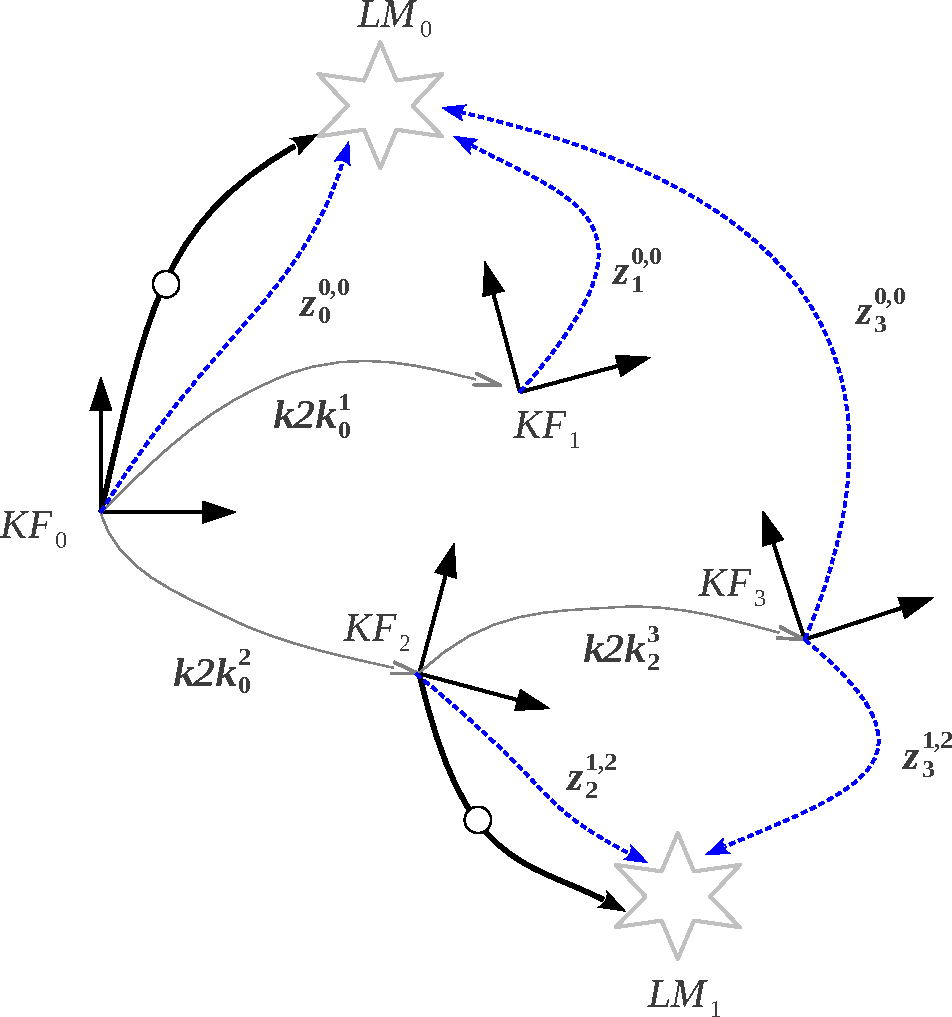
\includegraphics[width=0.7\textwidth]{imgs/srba_toy_problem.pdf} 
\caption{A toy RBA problem.}
\label{fig:rba.entities}
\end{figure}

An example such that the one in Fig.~\ref{fig:rba.entities} will help introducing the different elements.
The illustration depicts many elements, some of which are \emph{known} data, others are the problem \emph{unknowns}. 
The goal of RBA is to recover a \emph{maximum-likelihood estimation (MLE)} of those unknowns. Optionally, the covariances and 
cross-covariances between estimated variables can be also evaluated.

We find the following entities in \texttt{libmrpt-srba} (refer to Fig.~\ref{fig:rba.entities}):

\begin{itemize}
\item{\textbf{Keyframes}: A keyframe (KF), as each $KF_i$ in the figure, represents the \emph{pose} of the robot (or the 
camera or whatever) at one  particular instant of time. In RBA we will never work with the absolute coordinates of any of 
these KFs. This is completely different than ``common'' Bundle Adjustment, where these poses are the unknowns to 
estimate.
}
\item{\textbf{Keyframe-to-keyframe (k2k) edges}: An edge $k2k_i^j$ represents the relative pose of $KF_i$ with respect to 
$KF_j$. Notice that ``inverse poses'' (i.e. in the inverse order than one would expect from the edge direction) are 
stored for efficiency\footnote{In RBA we may need to chain sequences of relative poses and the direction will often 
be from newer KFs towards older KFs, hence if we store inverse poses we save the computational burden of inverting them 
over and over again.}. These edges are always treated as \emph{unknowns} to be estimated from observation data.
They can be parameterized in different ways (see \S\ref{sec:k2k_types}), but the two choices in practice are 
either SE(2) or SE(3) poses.
}
\item{\textbf{Landmarks}: A landmark (LM) is any entity which can be observed from different locations. Typically a 2D 
or 3D point in space, but could be a line, segment, plane or any user-defined entity. They are represented in 
the Fig.~\ref{fig:rba.entities} as stars denoted as $LM_i$. The concept of absolute coordinates of a LM 
does not exist in RBA.
}
\item{\textbf{Relative position and "base keyframe" of a LM}: Each LM is associated to exactly one KF, its {base KF}, with 
respect to which the LM has a \emph{relative position}. This relative position can be either ``known'' (``\emph{fixed}'' 
in the C++ API) or ``unknown'', in which case it is also estimated during the problem optimization. There exist several 
possible ways of parameterizing relative positions, as discussed in \S\ref{sec:k2f_types}. These relative positions are 
represented in the figure as thick edges with circle marks in the middle.
}
\item{\textbf{Observations}: An observation $z^{i,j}_k$ stands for any piece of sensory data which \emph{is related}, 
somehow, with the position of the $i-th$ LM, whose base KF is $j$, as seen from the observing KF $k$. They are 
depicted as dashed lines in the figure above. Rank-deficient observations, like those from monocular cameras, are 
acceptable but two or more observations are then required before being able to estimate the relative position of the 
observed LM.
}
\end{itemize}


\newpage


\section{Programmer's first steps}
\label{sect:program_first}

The central class in \texttt{libmrpt-srba} is the template \texttt{RbaEngine<>}, which 
adopts a ``policy-based design'' \cite{andrei2001modern}:

\begin{lstlisting}
template <
	class KF2KF_POSE_TYPE,
	class LM_TYPE,
	class OBS_TYPE, 
	class RBA_OPTIONS = RBA_OPTIONS_DEFAULT>
class RbaEngine;
\end{lstlisting}

Thus, by setting each of the \emph{template arguments} we literally control the process 
of code generation to address one particular instance of a RBA problem. 
Since all this happens at \emph{compile time}, the compiler produces optimized code for 
the problem at hand (e.g. SSE2 code for multiplying matrices of a particular size), 
avoids code bifurcations, etc.

Due to the combinatorial nature of all the possibilities, 
detailed in \S\ref{sect:rba_configs}, one template class 
can generate specialized code for dozens of concrete problems, 
including new ones defined by the user without modifying the library at all.
The only price to pay is the longer compiling time associated to any complex C++ program 
that exploits metaprogramming with templates.


\subsection{The simplest program}

The following code illustrates the declaration of an RBA problem for 3D point landmarks, 
with SE(3) relative poses for keyframes and 3D range-bearing observations. 
Only two keyframes are defined, which means that after introducing the second one
there will be only one k2k edge (an unknown), which will be estimated by the least-squares 
optimizer along the relative positions of all landmarks.

\begin{lstlisting}
#include <mrpt/srba.h>

using namespace mrpt::srba;
using namespace std;

typedef RbaEngine<
	kf2kf_poses::SE3,       // Parameterization  KF-to-KF poses
	landmarks::Euclidean3D, // Parameterization of landmark positions    
	observations::RangeBearing_3D // Type of observations
	>
	my_srba_t;

int main(int argc, char**argv)
{
	my_srba_t rba;  //  Create an empty RBA problem
	
	// Define observations of KF #0:
	// ----------------------------------------------
	my_srba_t::new_kf_observations_t  list_obs;
	my_srba_t::new_kf_observation_t   obs_field;
	obs_field.is_fixed = false; // Landmarks have unknown relative 
	                            // positions (i.e. are unknowns )
	obs_field.is_unknown_with_init_val = false; // We don't have 
       // any guess on the initial LM position (will invoke the 
       // inverse sensor model)

	// For each observation:
	for (...) {
		obs_field.obs.feat_id = ...; // The landmark ID
		obs_field.obs.obs_data.range = ...;
		obs_field.obs.obs_data.yaw   = ...;
		obs_field.obs.obs_data.pitch = ...;
		list_obs.push_back( obs_field );
	}

	//  This is the main API entry point: Define KF #0
	my_srba_t::TNewKeyFrameInfo new_kf_info; // Placeholder of out info.
	rba.define_new_keyframe(
		list_obs,      // Input observations for the new KF
		new_kf_info,   // Output info
		true           // Run optimization of the local area
		);

	// Define observations of KF #1:
	// ----------------------------------------------
	list_obs.clear();
	// For each observation:
	for (...) {
		obs_field.obs.feat_id = ...; // The landmark ID
		obs_field.obs.obs_data.range = ...;
		obs_field.obs.obs_data.yaw   = ...;
		obs_field.obs.obs_data.pitch = ...;
		list_obs.push_back( obs_field );
	}

	//  This is the main API entry point: Define KF #1
	rba.define_new_keyframe(
		list_obs,      // Input observations for the new KF
		new_kf_info,   // Output info
		true           // Run optimization of the local area
		);

	cout << "Created KF #" << new_kf_info.kf_id 
	 << " | # kf-to-kf edges created:" <<  
	 new_kf_info.created_edge_ids.size() << endl <<
	 "Optimization error: " << 
	 new_kf_info.optimize_results.total_sqr_error_init << 
	 " -> " << 
	 new_kf_info.optimize_results.total_sqr_error_final << endl;

	// Save RBA graph as Graphviz file:
	rba.save_graph_as_dot("graph.dot", true /* LMs=save */);

	return 0;
}
\end{lstlisting}

\newpage

\subsection{API entry points}

It must be highlighted that, at present, the only API for inserting new KFs 
into the RBA problem is the method \texttt{define\_new\_keyframe()}:

\begin{lstlisting}
template <...> class RbaEngine {
    ...
	void define_new_keyframe(
		const typename traits_t::new_kf_observations_t  & obs,
		TNewKeyFrameInfo  & out_new_kf_info,
		const bool        run_local_optimization = true
		);
    ...
};
\end{lstlisting}

\noindent which accepts as its main input the list of all the observations gathered at this 
new KF. This method \emph{always creates a new KF}, without analyzing whether it was 
too close or too far from other KFs. Thus, it is (for now) the user's responsibility 
not to call the method too often, which would create an unnecessarily large amount of KFs with 
the subsequent degradation of the performance. \emph{The constant-time complexity} of the overall 
method assumes that there exists a maximum number of KFs per area --which is perfectly reasonable\footnote{TO DO: Future
versions of the software will probably incorporate an automatic mechanism to help deciding whether to insert
KFs.}.

As output, this method fills a 
\href{http://reference.mrpt.org/svn/structmrpt_1_1srba_1_1_rba_engine_1_1_t_new_key_frame_info.html}
{\texttt{RbaEngine<>::TNewKeyFrameInfo}} 
structure with:
\begin{itemize}
 \item The ID of the newly-created KF. 
 \item{ The list of all the created KF-to-KF edges. At least one, or more in the case of loop-closures. 
        The way in which edges are created depends on the \emph{edge-creation policy} (see \S\ref{sect:edge.policy}).
        An exception will be raised if no suitable edge is found to connect the new KF to the existing graph.}
 \item The numerical results from the local optimization process: the exact list of unknowns that undergone optimization, 
       the initial and final root mean-squared error (RMSE), etc.
\end{itemize}

Please, refer to the pseudocode description of this method 
in \S\ref{sect:code:define_new_keyframe} for a better insight of 
what happens inside.


\newpage

\subsection{Tutorials}

More complete versions of the program above, including sample datasets and rendering of the optimization result 
as OpenGL scenes are shipped with the source code\footnote{See the directory \texttt{[MRPT]/samples/srba-examples/srba-tutorials/}, 
or \href{http://mrpt.googlecode.com/svn/trunk/samples/srba-examples/srba-tutorials/}{browse online}.}.
Screenshots are shown in Figs.~\ref{fig:screenshot.tutorial1}--\ref{fig:screenshot.tutorial2}.

\begin{figure}[h]
\centering
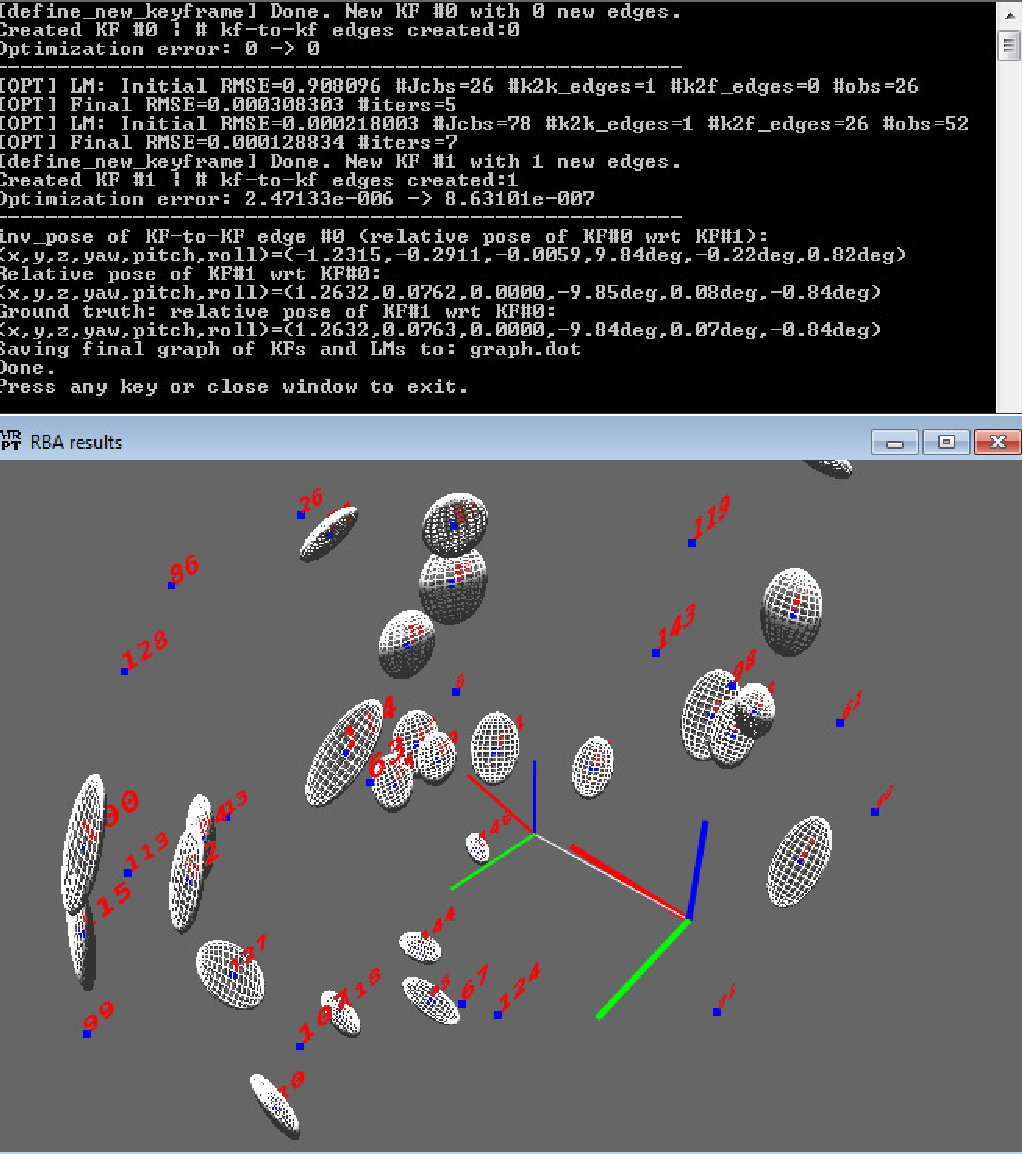
\includegraphics[width=0.9\textwidth]{imgs/screenshot_tutorial_range-bearing-3D.pdf} 
\caption{Screenshot for \texttt{tutorial-srba-range-bearing-se3.cpp}. Only two KFs are defined in this example.}
\label{fig:screenshot.tutorial1}
\end{figure}

\newpage

\begin{figure}[h]
\centering
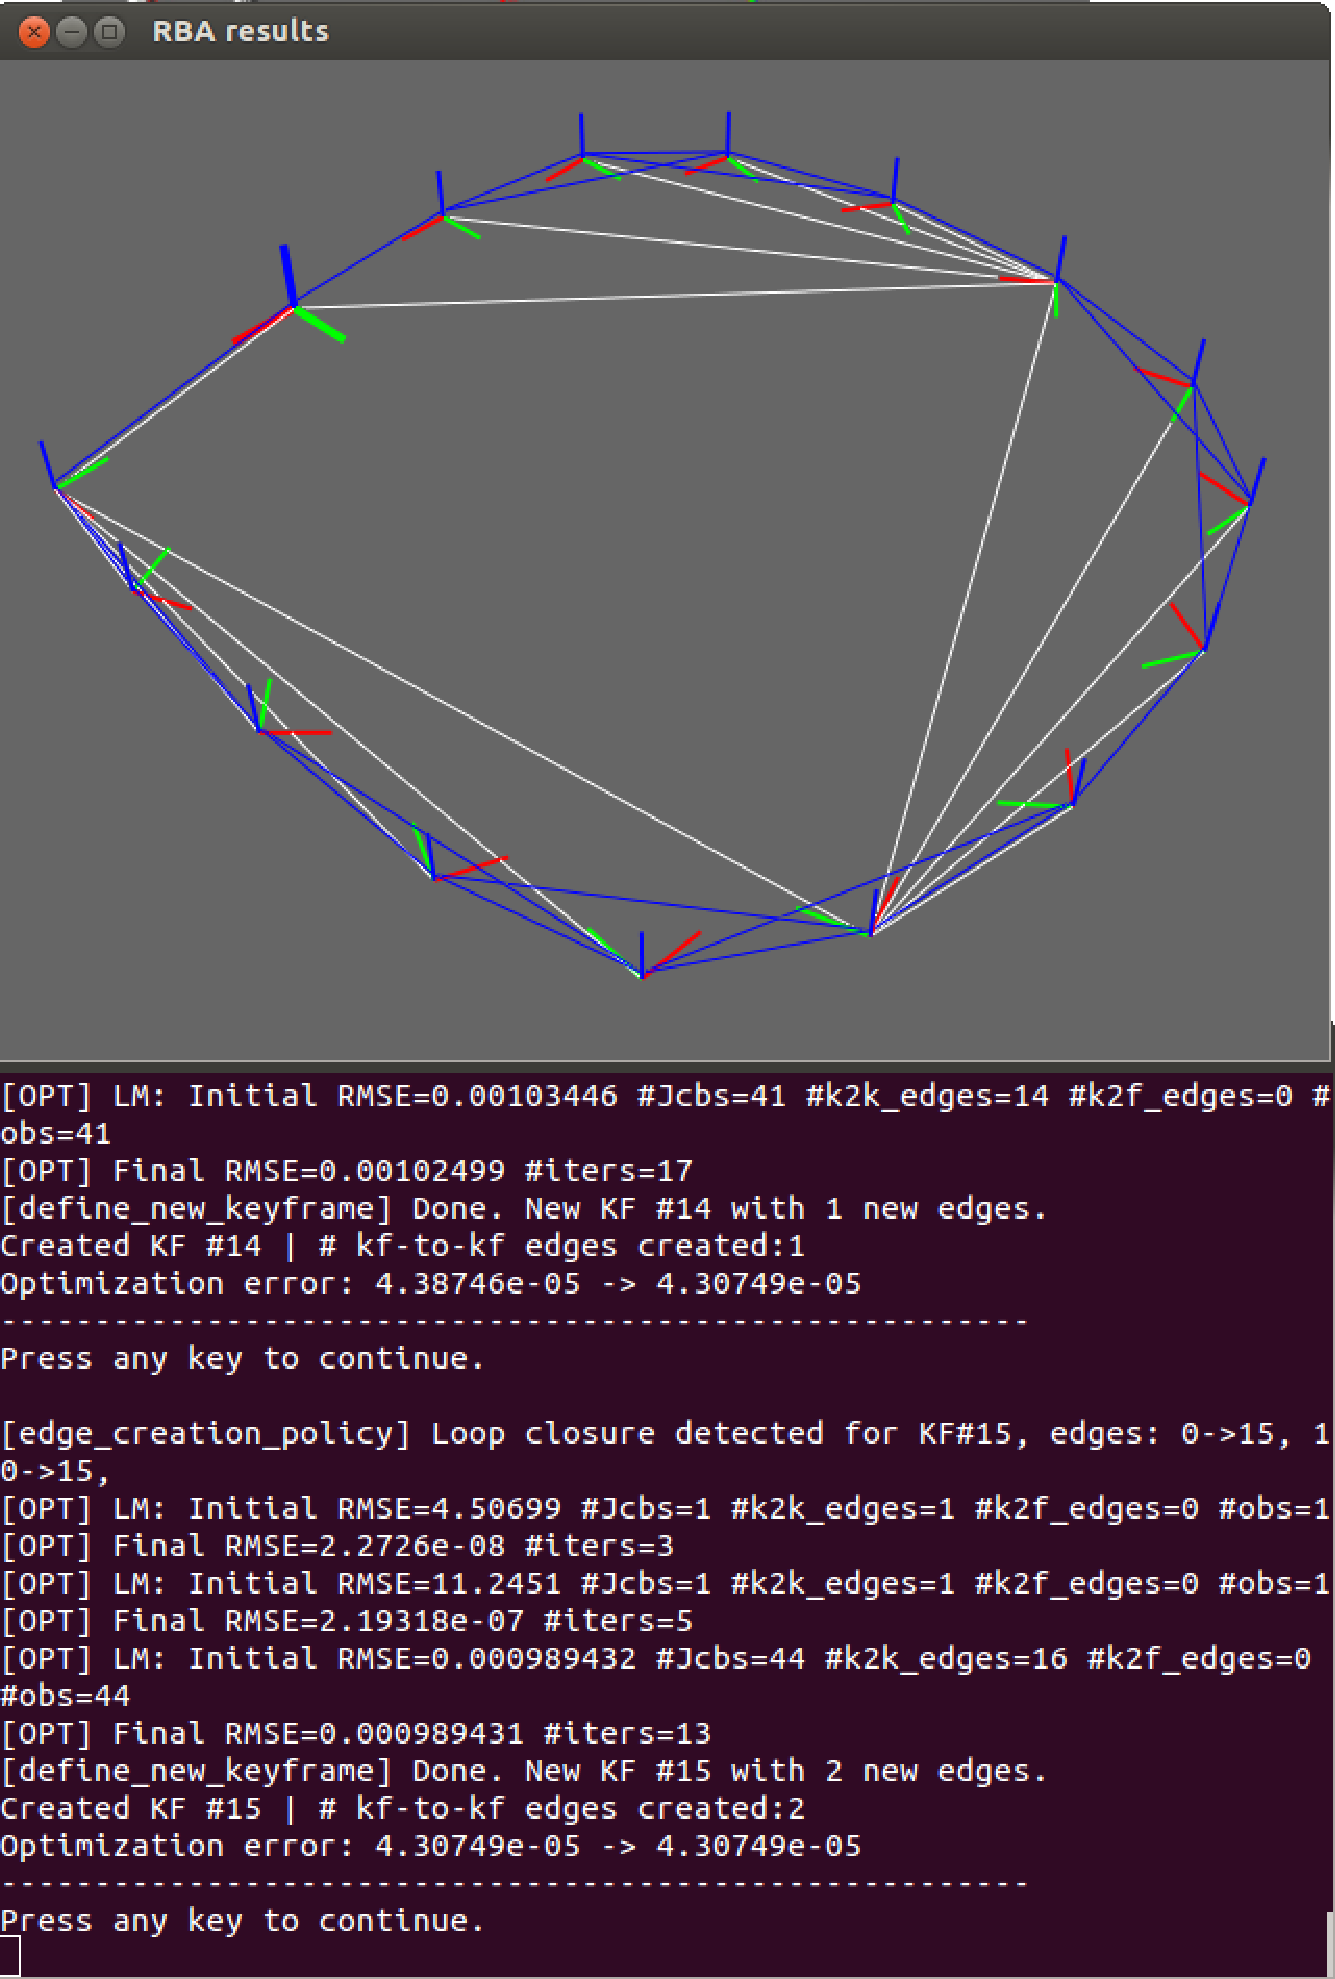
\includegraphics[width=0.75\textwidth]{imgs/screenshot_tutorial_relative-graph-slam-2D.pdf} 
\caption{Screenshot for \texttt{tutorial-srba-relative-graph-slam.cpp}. 
White lines represent KF-to-KF edges (unknowns), blue lines are observations (known data).}
\label{fig:screenshot.tutorial2}
\end{figure}

\newpage

\section{Configuring \texttt{RbaEngine<>}: template arguments}
\label{sect:rba_configs}

In the following, all class names assume the existence of a previous:

\begin{lstlisting}
 using namespace mrpt::srba;
\end{lstlisting}



\subsection{\texttt{KF2KF\_POSE\_TYPE}: KF-to-KF relative poses}
\label{sec:k2k_types}

This template argument selects the model for the relative poses between keyframes. 
The two natural possibilities are SE(2) and SE(3) poses, which you should employ 
depending on whether your problem can be considered \emph{planar} or not:

\begin{itemize}
\item{\textbf{ \texttt{kf2kf\_poses::SE2} }: For 2D relative poses, i.e. they consists of a $(x,y)$ displacement 
plus a heading $\phi$. Poses are mapped to 
\href{http://reference.mrpt.org/stable/classmrpt_1_1poses_1_1_c_pose2_d.html}
{\texttt{mrpt::poses::CPose2D}} classes. 
}
\item{\textbf{ \texttt{kf2kf\_poses::SE3} }: For 3D relative poses. Given that the least-squares optimization runs 
on the linearized neighborhood of the manifold \cite{blanco2010tutorial} around the instantaneous solutions, the 
choice between different parameterizations (i.e. quaternions, Euler angles,etc.) becomes irrelevant. 
In this case poses become 
\href{http://reference.mrpt.org/stable/classmrpt_1_1poses_1_1_c_pose3_d.html}
{\texttt{mrpt::poses::CPose3D}}
classes, which internally hold the $3 \times 3$ rotation matrices for SO(3) rotations and $(x,y,z)$ vectors 
for the translational parts, with optional conversion to/from quaternions and yaw/pitch/roll angles.
}
\end{itemize}

Notice that the usage of 2D relative poses limits the robot trajectory to one single plane, but 
does not restrict landmarks to also be planar. 
It is perfectly legal to use planar poses and 3D landmarks.


\subsection{\texttt{LM\_TYPE}: Relative landmark parameterizations}
\label{sec:k2f_types}

\begin{itemize}
\item{\textbf{ \texttt{landmarks::Euclidean2D} }: Point landmarks, parameterized with 2D Euclidean coordinates with respect to the base KF.
}
\item{\textbf{ \texttt{landmarks::Euclidean3D} }: Point landmarks, parameterized with 3D Euclidean coordinates with respect to the base KF.
}
\item{\textbf{ \texttt{landmarks::RelativePoses2D} }: A kind of ``fake landmark'' used in relative graph-SLAM. 
Represents the pose of the base KF, which can be observed from another KF.}
\end{itemize}

The implementation of these models can be seen in:

\texttt{\#include <mrpt/srba/models/landmarks.h>}.

\vspace{1cm}
\subsection{\texttt{OBS\_TYPE}: Observation types}

The following observations are implemented and ready to use in the library:

\begin{itemize}
\item{\textbf{ \texttt{observations::MonocularCamera} }: A pair of pixel coordinates $(x,y)$ for the observed landmark.}
\item{\textbf{ \texttt{observations::StereoCamera} }: Pixel coordinates for one left and one right camera.}
\item{\textbf{ \texttt{observations::Cartesian\_2D} }: The $(x,y)$ coordinates of the observed landmark, relative to the sensor.}
\item{\textbf{ \texttt{observations::Cartesian\_3D} }: The $(x,y,z)$ coordinates of the observed landmark, relative to the sensor.}
\item{\textbf{ \texttt{observations::RangeBearing\_2D} }: The distance and the angle (polar coordinates) of the observed landmark, relative to
the sensor.}
\item{\textbf{ \texttt{observations::RangeBearing\_3D} }: The distance and two angles (yaw and pitch) of the observed landmark, relative
to the sensor.}
\item{\textbf{ \texttt{observations::RelativePoses\_2D} }: The $(x,y,\phi)$ pose of the observed KF, relative to the observer KF.}
\end{itemize}

The implementation of these models can be seen in:

\texttt{\#include <mrpt/srba/models/observations.h>}.


\subsection{Sensor models}
\label{sect:program_sensors}

In order to use together each combination of landmark parameterization (\texttt{LM\_TYPE}) and 
observation (\texttt{OBS\_TYPE}) a correct \emph{sensor model} must be implemented which 
takes care of providing a set of Jacobians, an inverse sensor model, etc.

These are the models already implemented with this library: 

\begin{itemize}
\item{\textbf{ \texttt{landmarks::Euclidean3D + observations::MonocularCamera}}: 3D landmarks in Euclidean coordinates, observed 
with a monocular camera (without distortion).}
\item{\textbf{ \texttt{landmarks::Euclidean3D + observations::StereoCamera}}: 3D landmarks in Euclidean coordinates, observed 
with a stereo camera (without distortion).}
\item{\textbf{ \texttt{landmarks::Euclidean2D + observations::Cartesian\_2D}}: 2D landmarks in Euclidean coordinates, whose
Euclidean coordinates are directly observed.}
\item{\textbf{ \texttt{landmarks::Euclidean3D + observations::Cartesian\_3D}}: 3D landmarks in Euclidean coordinates, whose
Euclidean coordinates are directly observed.}
\item{\textbf{ \texttt{landmarks::Euclidean2D + observations::RangeBearing\_2D}}: 2D landmarks in Euclidean coordinates, observed
via range and bearing.}
\item{\textbf{ \texttt{landmarks::Euclidean3D + observations::RangeBearing\_3D}}: 3D landmarks in Euclidean coordinates, observed
via range and bearing.}
\item{\textbf{ \texttt{landmarks::RelativePoses2D + observations::RelativePoses\_2D}}: The sensor model for 2D relative graph-SLAM.}
\end{itemize}

The implementation of these models can be seen in:

\texttt{\#include <mrpt/srba/models/sensors.h>}.


\subsection{\texttt{RBA\_OPTIONS}: Other options}
\label{sect:rba_options}

This template argument must be a user-defined structure with a set of \texttt{typedef}s 
that configure specific aspects of the RBA problem, explored below:

\begin{lstlisting}
struct my_rba_options
{
  typedef <TYPE_1>  sensor_pose_on_robot_t;
  typedef <TYPE_2>  obs_noise_matrix_t;
  typedef <TYPE_3>  solver_t;
};
\end{lstlisting}


\subsubsection{Choices for \texttt{sensor\_pose\_on\_robot\_t}}

\begin{itemize}
\item{\textbf{ \texttt{options::sensor\_pose\_on\_robot\_none}}: The pose of a KF corresponds exactly to the pose of the 
sensor. That is, 
there is no distinction between the pose of the ``robot'' and that of the ``sensor''.}
\item{\textbf{ \texttt{options::sensor\_pose\_on\_robot\_se3}}: The sensor is located at an arbitrary pose with respect to 
the frame of reference of each KF (the ``robot''). This is the most common case of sensors placed on a mobile robot, 
and should be used if we are interested in obtaining the pose of the robot instead of that of the sensor itself. 
In the case of cameras, this option is employed within the program \texttt{srba-slam} to establish a change of coordinates
between the Z-points-up standard for robot poses and the Z-points-forward of typical camera models. 
Using this option has a small computational overhead in comparison to the one above.}
\end{itemize}

The list of possible types can be found in: 

\texttt{\#include <mrpt/srba/srba\_options\_sensor\_pose.h>}.


\subsubsection{Choices for \texttt{obs\_noise\_matrix\_t}}

This option controls the way in which the information matrix $\boldsymbol \Lambda_k$ for the $k-th$ observation 
(inverse of the sensor error
covariance matrix) is incorporated into the weighted least-squares optimizer.
Depending on the chosen model, different data fields to set the model parameters 
will be available under \texttt{srba.parameters.obs\_noise}.

\begin{itemize}
\item{\textbf{ \texttt{options::observation\_noise\_identity}}: 
This is the most computationally efficient method, since it is assumed that:
  \begin{equation}
  \boldsymbol \Lambda_k = \Lambda \mathbf{I}
  \end{equation}
\noindent with $\mathbf{I}$ an identity matrix of the correct size. 
The error is exactly the same for all observations.}

\item{\textbf{ \texttt{options::observation\_noise\_constant\_matrix}}: 
In this case $\boldsymbol \Lambda_k$ can be any arbitrary matrix\footnote{As long
as it is a valid information matrix: symmetric, positive definite.}. The same 
matrix will be used for all observations.}

\end{itemize}

The list of possible types can be found in: 

\texttt{\#include <mrpt/srba/srba\_options\_sensor\_noise.h>}.


\subsubsection{Choices for \texttt{solver\_t}}
\label{sect:choices.solvers}

At present all solvers are different versions of the Levenberg-Marquardt (LM) algorithm:

\begin{itemize}
\item{\textbf{ \texttt{options::solver\_LM\_schur\_dense\_cholesky}}: A LM solver, 
using the Sch\"ur complement to build a reduced system of equations for relative poses only, 
which is then solved using a dense Cholesky factorization.}

\item{\textbf{ \texttt{options::solver\_LM\_schur\_sparse\_cholesky}}: Like above, but 
using a sparse Cholesky factorization (with the \texttt{CSparse} library) for the reduced system.}

\item{\textbf{ \texttt{options::solver\_LM\_no\_schur\_sparse\_cholesky}}: A LM solver,
directly using a sparse Cholesky factorization (with the \texttt{CSparse} library) on 
the entire system of equations (both poses and landmarks).}

\end{itemize}

The list of possible types can be found in: 

\texttt{\#include <mrpt/srba/srba\_options\_solver.h>}.


\section{Configuring \texttt{RbaEngine<>}: dynamic parameters}
\label{sect:rba_dyn_parameters}

In contrast to the template arguments, which determine the type of problem at compile time, 
there exist another set of parameters, suitable for change at run-time.

They are all found in the public field \texttt{parameters}, which 
in turn is built up of other \texttt{struct}s whose contents are determined
at compile time depending on the template arguments:

\begin{lstlisting}
template <...> class RbaEngine {
  ...
  struct TAllParameters
  {
    /** Different parameters for the SRBA methods */
    TSRBAParameters  srba;

    /** Sensor-specific parameters (sensor calibration, etc.) */
    typename OBS_TYPE::TObservationParams   sensor;

    /** Parameters related to the relative pose of sensors wrt the robot (if applicable) */
    typename RBA_OPTIONS::sensor_pose_on_robot_t::parameters_t  sensor_pose;

    /** Parameters related to the sensor noise covariance matrix */
    typename RBA_OPTIONS::obs_noise_matrix_t::parameters_t  obs_noise;
  };

  TAllParameters parameters;
  ...
};
\end{lstlisting}

  
\subsection{Depth of spanning trees}

Two of the most important parameters are:

\begin{lstlisting}
template <...> class RbaEngine {
  ...
  struct TSRBAParameters
  {
  ...
  /** Maximum depth for maintained spanning trees. */
  topo_dist_t          max_tree_depth;
  /** The maximum topological distance of keyframes 
     to be optimized around the most recent keyframe. */
  topo_dist_t          max_optimize_depth;
  ...
  };
  ...
};
\end{lstlisting}

In general, \texttt{parameters.srba.max\_optimize\_depth} should not be larger than 
\texttt{parameters.srba.max\_tree\_depth}, 
since optimization needs using the prebuilt spanning trees. Normally, both values will be the same and very small (e.g. 3 or 4).

\subsection{Edge-creation policy}
\label{sect:edge.policy}

Another critical parameter is:

\begin{lstlisting}
template <...> class RbaEngine {
  ...
  struct TSRBAParameters
  {
  ...
    TEdgeCreationPolicy edge_creation_policy;
  ...
  };
  ...
};
\end{lstlisting}

Here, \texttt{parameters.srba.edge\_creation\_policy} controls the policy 
to decide, given a set of observations for a new KF, 
how many KF-to-KF edges must be created and how should they be connected.

Check the doxygen documentation for 
\href{http://reference.mrpt.org/svn/namespacemrpt_1_1srba.html#af0fbe388a6a76d59f66e7b8d1353926c}
{\texttt{TEdgeCreationPolicy}} for a description of the possibilities.

Note that the user can implement new custom policies by overriding the virtual method:

\begin{lstlisting}
template <...> class RbaEngine {
  ...
  virtual void edge_creation_policy(
    const TKeyFrameID               new_kf_id,
    const typename traits_t::new_kf_observations_t   & obs,
    std::vector<TNewEdgeInfo> &new_k2k_edge_ids );
  ...
};
\end{lstlisting}

\noindent in which case the value of 
\texttt{parameters.srba.edge\_creation\_policy}
is ignored.


\newpage
\subsection{Levenberg-Marquardt solver parameters}
\label{sect:lm-params}

All these can be found under
\texttt{parameters.srba.*}:


\subsubsection{Fluid relinearization}

\textbf{\texttt{double min\_error\_reduction\_ratio\_to\_relinearize}:} If the error-reduction ratio 
between two consecutive solver iterations is below this threshold, Jacobians will not be re-evaluated 
at the new solution. This a kind of ``fluid relinearization'', which reduces the computational burden.

\subsubsection{Covariance recovery}

\textbf{\texttt{TCovarianceRecoveryPolicy  cov\_recovery}:} Controls how or whether covariances 
are to be recovered from the final Hessian matrix used by the solver. Naive exact recovery implies 
inverting a sparse matrix, leading to a dense (fully-correlated) covariance matrix, which is normally expensive.
That is why, by default, only an approximation of the landmark covariances are evaluated.
See the Doxygen documentation for 
\href{http://reference.mrpt.org/svn/namespacemrpt_1_1srba.html#a14e4d971f53601c3b72ba1a321e7b9e1}
{\texttt{TCovarianceRecoveryPolicy}}
for further details.

Note that the Hessian itself (i.e. the sparse inverse of the covariance of all unknowns) 
is also always provided in the member \texttt{extra\_results}:

\begin{lstlisting}
template <...> class RbaEngine {
  ...
  struct TOptimizeExtraOutputInfo 
  {
    ...
    typename RBA_OPTIONS::solver_t::extra_results_t   extra_results; 
    ...
  };
  ...
};
\end{lstlisting}

\noindent after each successful optimization. 
The specific format in which this Hessian is provided (i.e. sparse vs. dense) depends on the selected solver 
(see \S\ref{sect:choices.solvers}). 
The user can apply any advanced algorithm for recovering only the part of the covariances really required 
for the application at hand.

\newpage
\subsubsection{Others}

These other parameters are also worth mentioning:

\begin{itemize}
\item{\textbf{\texttt{bool optimize\_new\_edges\_alone}:} Runs an optimization with the new KF-to-KF edges, 
one by one, as if they were the unique unknowns before running the local area optimization. This assures 
that there are no variables with such a bad initialization that could ruin the overall estimation. 
Normally should be left to \texttt{true}, disable for a speed up if you are sure this step is not needed 
in your problem. }

\item{\textbf{\texttt{bool use\_robust\_kernel}:} Employs a robustifying kernel (pseudo-Huber) to reduce the 
impact of outliers. Enabled by default. Should also tune the \texttt{kernel\_param} parameter.}

\item{\textbf{\texttt{size\_t max\_iters}:} Maximum number of iterations in the least-squares solver.}
\end{itemize}


\newpage
\section{Accessing \texttt{RbaEngine<>}: the RBA problem graph}
\label{sect:rba_access}

This section is meant to be complemented by checking the complete Doxygen documentation online.

\subsection{Programmatic access to edges and nodes}

The first step for programmatic access to the data structures that 
represent KFs, observations, etc. is getting a (\texttt{const}, i.e. unmodifiable) 
reference to the internal object that holds the entire RBA state:

\begin{lstlisting}
template <...> class RbaEngine {
    ...
	typedef TRBA_Problem_state<...> rba_problem_state_t;
	...
	const rba_problem_state_t & get_rba_state() const;
    ...
};
\end{lstlisting}

\noindent which is an instance of the class 
\href{http://reference.mrpt.org/svn/structmrpt_1_1srba_1_1_t_r_b_a___problem__state.html}
{\texttt{TRBA\_Problem\_state<...>}}. It is recommended to check its Doxygen documentation
for a better description of all the existing data fields, as well as the description in \S\ref{sect:data.structs}.
The most relevant public data fields are:
\begin{itemize}
\item \texttt{keyframe\_vector\_t keyframes}: A vector with information about each existing KF, indexed by their ID.
\item \texttt{k2k\_edges\_deque\_t k2k\_edges}: All KF-to-KF edges, indexed by their ID.
\item \texttt{TRelativeLandmarkPosMap unknown\_lms}: The positioning of each (non-fixed) landmark.
\end{itemize}


\newpage
\subsection{Exporting as OpenGL objects}

The following method is provided to convert (part of) an RBA problem into a graphical representation 
suitable for rendering:

\begin{lstlisting}
template <...> class RbaEngine {
    ...
	void build_opengl_representation(
		const srba::TKeyFrameID root_keyframe,
		const TOpenGLRepresentationOptions &options,
		mrpt::opengl::CSetOfObjectsPtr out_scene,
		mrpt::opengl::CSetOfObjectsPtr out_root_tree = mrpt::opengl::CSetOfObjectsPtr()
		) const;
    ...
};
\end{lstlisting}

It is recommended to check the Doxygen documentation of 
\href{http://reference.mrpt.org/svn/structmrpt_1_1srba_1_1_rba_engine_1_1_t_open_g_l_representation_options.html}
{\texttt{TOpenGLRepresentationOptions}} to see all available rendering options, but just a few important remarks:

\begin{itemize}
\item{ In RBA there is no ``global map'', obviously. So each graphical representation must explicitly choose the 
       origin of coordinates. This is done by selecting the \texttt{root\_keyframe} (a KF's ID) which becomes the 
       root of a spanning tree of all nearby KFs up to some maximum topological distance (settable in \texttt{options}).}
\item{ For obtaining relative coordinates with respect to the selected root, this method is capable of building deeper
       spanning trees than those maintained for online optimization. However, this clearly has an unbounded computational 
       cost that grows with the desired topological distance, so keep this distance as reduced as possible if the intention 
       is to render the state of the RBA problem in real time. In particular, it is recommended to set: 

\begin{lstlisting}
	typename my_srba_t::TOpenGLRepresentationOptions opengl_params;
	opengl_params.span_tree_max_depth = rba.parameters.srba.max_tree_depth; // Render these past keyframes at most.
\end{lstlisting}
}
\end{itemize}

\newpage
\subsection{Exporting as Graphviz graphs}

The following method allows exporting the RBA problem, in its current state, to a plain text 
file in the standard Graphviz format:

\begin{lstlisting}
template <...> class RbaEngine {
    ...
	bool save_graph_as_dot(
		const std::string &targetFileName,
		const bool all_landmarks = false
		) const;
    ...
};
\end{lstlisting}

Note that exporting all landmarks will lead to excessively dense graphs in any mid to large-size problem. 
An example is shown in Fig.~\ref{fig:dot.graph}.

\begin{figure}[h]
\centering
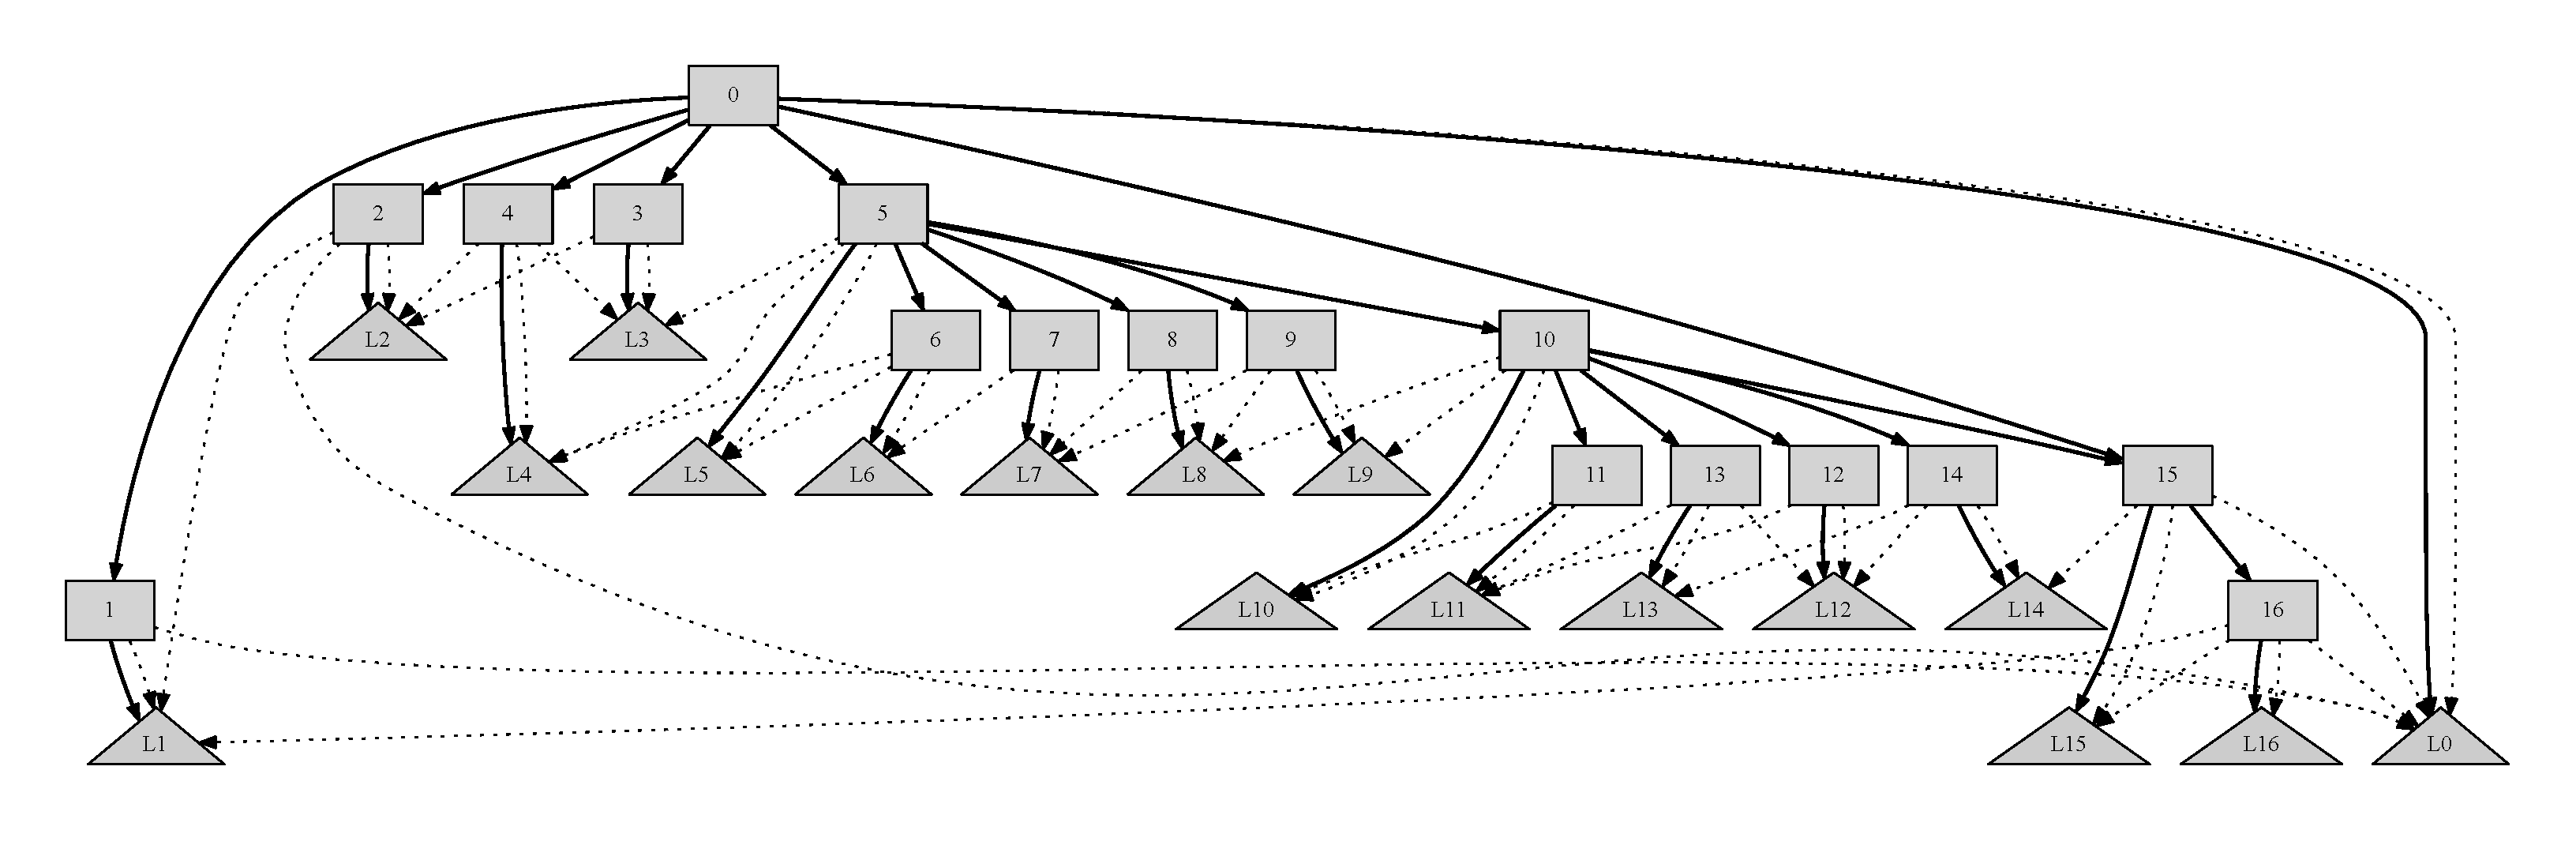
\includegraphics[width=1.0\textwidth]{imgs/example_final_graph.pdf} 
\caption{Example of an RBA graph rendered with Graphviz's \texttt{dot}: rectangles are keyframes, triangles are landmarks, 
dotted lines are observations and solid lines are either kf-to-kf edges or landmark relative positions 
(with respect to their \emph{base} keyframes).}
\label{fig:dot.graph}
\end{figure}

\newpage
\subsection{Generic graph visitor}

There exists a fully-customizable breadth-first search (BFS) \emph{visitor}, which allows any user-supplied 
class to process every node and edge in the RBA graph, starting at a given root KF 
and expanding in a classic breadth-first fashion:

\begin{lstlisting}
template <...> class RbaEngine {
    ...
	template <
		class KF_VISITOR,
		class FEAT_VISITOR,
		class K2K_EDGE_VISITOR,
		class K2F_EDGE_VISITOR
		>
	void bfs_visitor(
		const TKeyFrameID  root_id,
		const topo_dist_t  max_distance,
		const bool rely_on_prebuilt_spanning_trees,
		KF_VISITOR       & kf_visitor,
		FEAT_VISITOR     & feat_visitor,
		K2K_EDGE_VISITOR & k2k_edge_visitor,
		K2F_EDGE_VISITOR & k2f_edge_visitor ) const;
    ...
};
\end{lstlisting}

The option \texttt{rely\_on\_prebuilt\_spanning\_trees} is the only one requiring a few words.
It selects between two different ways of performing the BFS:
\begin{itemize}
 \item Relying on prebuilt spanning trees: such that the search is limited to the maximum depth of those trees, and 
 \item Not relying on them: then a complete BFS algorithm is run, suitable for exploration of the entire RBA problem graph.
\end{itemize}

The four template argument, the visitor classes, must be defined by the user. 
They may be four different classes or just one. 
Next follows a sketch of the expected minimum interface for each class:


\begin{lstlisting}
/* Implementation of FEAT_VISITOR */
struct MY_FEAT_VISITOR
{
	bool visit_filter_feat(
		const TLandmarkID lm_ID,
		const topo_dist_t cur_dist) 
	{
		// Return "true" if it's desired to visit this landmark node.
	}
	void visit_feat(
		const TLandmarkID lm_ID,
		const topo_dist_t cur_dist) 
	{
		// Process this landmark node.
	}
};
\end{lstlisting}
\begin{lstlisting}
/* Implementation of KF_VISITOR */
struct MY_KF_VISITOR
{
	bool visit_filter_kf(
		const TKeyFrameID kf_ID,
		const topo_dist_t cur_dist) 
	{
		// Return "true" if it's desired to visit this keyframe node.
	}
	void visit_kf(
		const TKeyFrameID kf_ID,
		const topo_dist_t cur_dist) 
	{
		// Process this keyframe node.
	}
};
\end{lstlisting}
\begin{lstlisting}
/* Implementation of K2K_EDGE_VISITOR */
struct MY_K2K_EDGE_VISITOR
{
	bool visit_filter_k2k(
		const TKeyFrameID current_kf, 
		const TKeyFrameID next_kf,
		const k2k_edge_t* edge, 
		const topo_dist_t cur_dist) 
	{
		// Return "true" if it's desired to visit this kf-to-kf edge.
	}
	void visit_k2k(
		const TKeyFrameID current_kf, 
		const TKeyFrameID next_kf,
		const k2k_edge_t* edge, 
		const topo_dist_t cur_dist)
	{
		// Process this kf-to-kf edge.
	}
};
\end{lstlisting}
\begin{lstlisting}
/* Implementation of K2F_EDGE_VISITOR */
struct MY_K2F_EDGE_VISITOR
{
	bool visit_filter_k2f(
		const TKeyFrameID current_kf, 
		const k2f_edge_t* edge, 
		const topo_dist_t cur_dist)
	{
		// Return "true" if it's desired to visit this kf-to-feat edge.
	}
	void visit_k2f(
		const TKeyFrameID current_kf, 
		const k2f_edge_t* edge, 
		const topo_dist_t cur_dist)
	{
		// Process this kf-to-feat edge.
	}
}; 
\end{lstlisting}




\newpage
\section{The \texttt{srba-slam} application}
\label{sect:srba_slam_app}

This program is ready to use in binary installations of MRPT, so it could be a good starting 
point to test the possibilities of SRBA without having to write a single line of code.

\subsection{Interface}

\texttt{srba-slam} is a command-line program that loads a dataset from plain text files 
and processes it with a given instance of the generic \texttt{RbaEngine}. 
A typical call must specify the desired models for relative poses, landmarks 
and observations, as well as the data set file:

\begin{lstlisting}
srba-slam {--se2|--se3} {--lm-2d|--lm-3d} --obs [StereoCamera|...]
          -d DATASET.txt [--sensor-params-cfg-file SENSOR_CONFIG.cfg]
          [--noise NOISE_SIGMA] [--verbose {0|1|2|3}] [--step-by-step]
\end{lstlisting}

The sensor configuration file (\texttt{--sensor-params-cfg-file }) is
only required for certain types of observations (e.g. camera calibration files
for vision sensors). 
Noise parameters can be provided via \texttt{--noise} (and \texttt{--noise-ang} for angular components) 
to modify the weighting of least squares optimization 
and, optionally (if \texttt{--add-noise} is set) actual random noise will be also generated and added to the dataset.

Naturally, not all possible RBA problems are precompiled in this
application. To see the list of available problems, run:

\begin{lstlisting}
srba-slam --list-problems
\end{lstlisting}


To explore all the existing parameters, please execute:

\begin{lstlisting}
srba-slam --help
\end{lstlisting}

\noindent or see the program man page:

\begin{lstlisting}
man srba-slam
\end{lstlisting}


\subsection{Running with sample datasets}

A small collection of datasets is shipped with MRPT and can be found under:

\begin{lstlisting}
[MRPT_ROOT]/share/mrpt/datasets/srba-demos/
\end{lstlisting}

\noindent where \texttt{[MRPT\_ROOT]} is: 
\begin{itemize}
 \item \texttt{C:/Program Files/MRPT/} if a Windows binary package was installed,
 \item \texttt{/usr/} if a GNU/Linux binary package was installed, or
 \item the root directory of source packages.
\end{itemize}

In all cases, shipped files are not the datasets themselves, but the \emph{sources}
for the RWT dataset generator\footnote{See: 
\href{http://code.google.com/p/recursive-world-toolkit/}{http://code.google.com/p/recursive-world-toolkit/}}. 
Follow instructions in the \texttt{README.txt} to generate the datasets. 

Then, see one of the \texttt{*.sh} files in the same directory for example calls to \texttt{srba-slam} for each dataset. 
As an example, this is how to run the 2D relative graph-SLAM dataset:


\begin{lstlisting}
srba-slam --se2 --graph-slam -d dataset_30k_rel_graph_slam_SENSOR.txt 
          --submap-size 10 
          --max-spanning-tree-depth 3 --max-optimize-depth 3
          --verbose 1 --noise 0.001 --noise-ang 0.2 --add-noise 
          --gt-map dataset_30k_rel_graph_slam_GT_MAP.txt 
          --gt-path dataset_30k_rel_graph_slam_GT_PATH.txt 
          # --step-by-step 
\end{lstlisting}



\newpage
\section{Spanning trees}

The need to hold spanning trees for every KF in the problem is motivated 
by the realization that \emph{topological paths} appear in the observation 
model of landmarks (or in that of relative poses in relative Graph-SLAM). 
In particular, we need the shortest path
between an observing KF and the base KF of the observed landmark, as highlighted 
in Figure~\ref{fig:STs1}.

\begin{figure}[h]
\centering
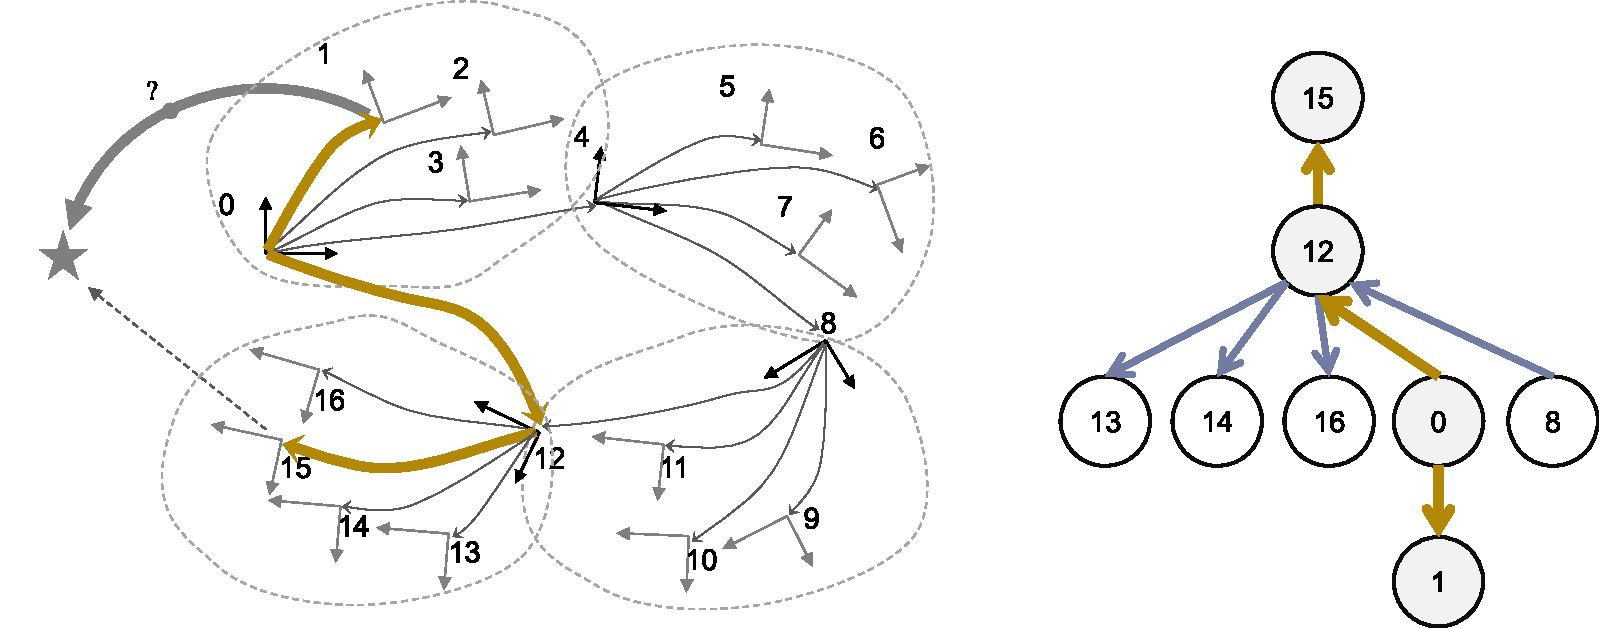
\includegraphics[width=1.0\textwidth]{imgs/spanning-tree-motivation1.pdf} 
\caption{(left) Paths between keyframes involved in observation models. (right) The corresponding spanning tree.}
\label{fig:STs1}
\end{figure}

Internally, each spanning tree is stored as a pair of sparse tables:
\begin{itemize}
 \item $ST.D[i][j]$: A symmetric table with the topological distance between keyframes $i \leftrightarrow j$.
 \item $ST.N[i][j]$: This table holds the next edge to follow if we are at $i$ and want to reach $j$. 
\end{itemize}

Our paper \cite{blanco2013srba} describes an algorithm for incrementally update those tables as new keyframes and edges
are added to the problem.

\begin{figure}[h!]
\centering
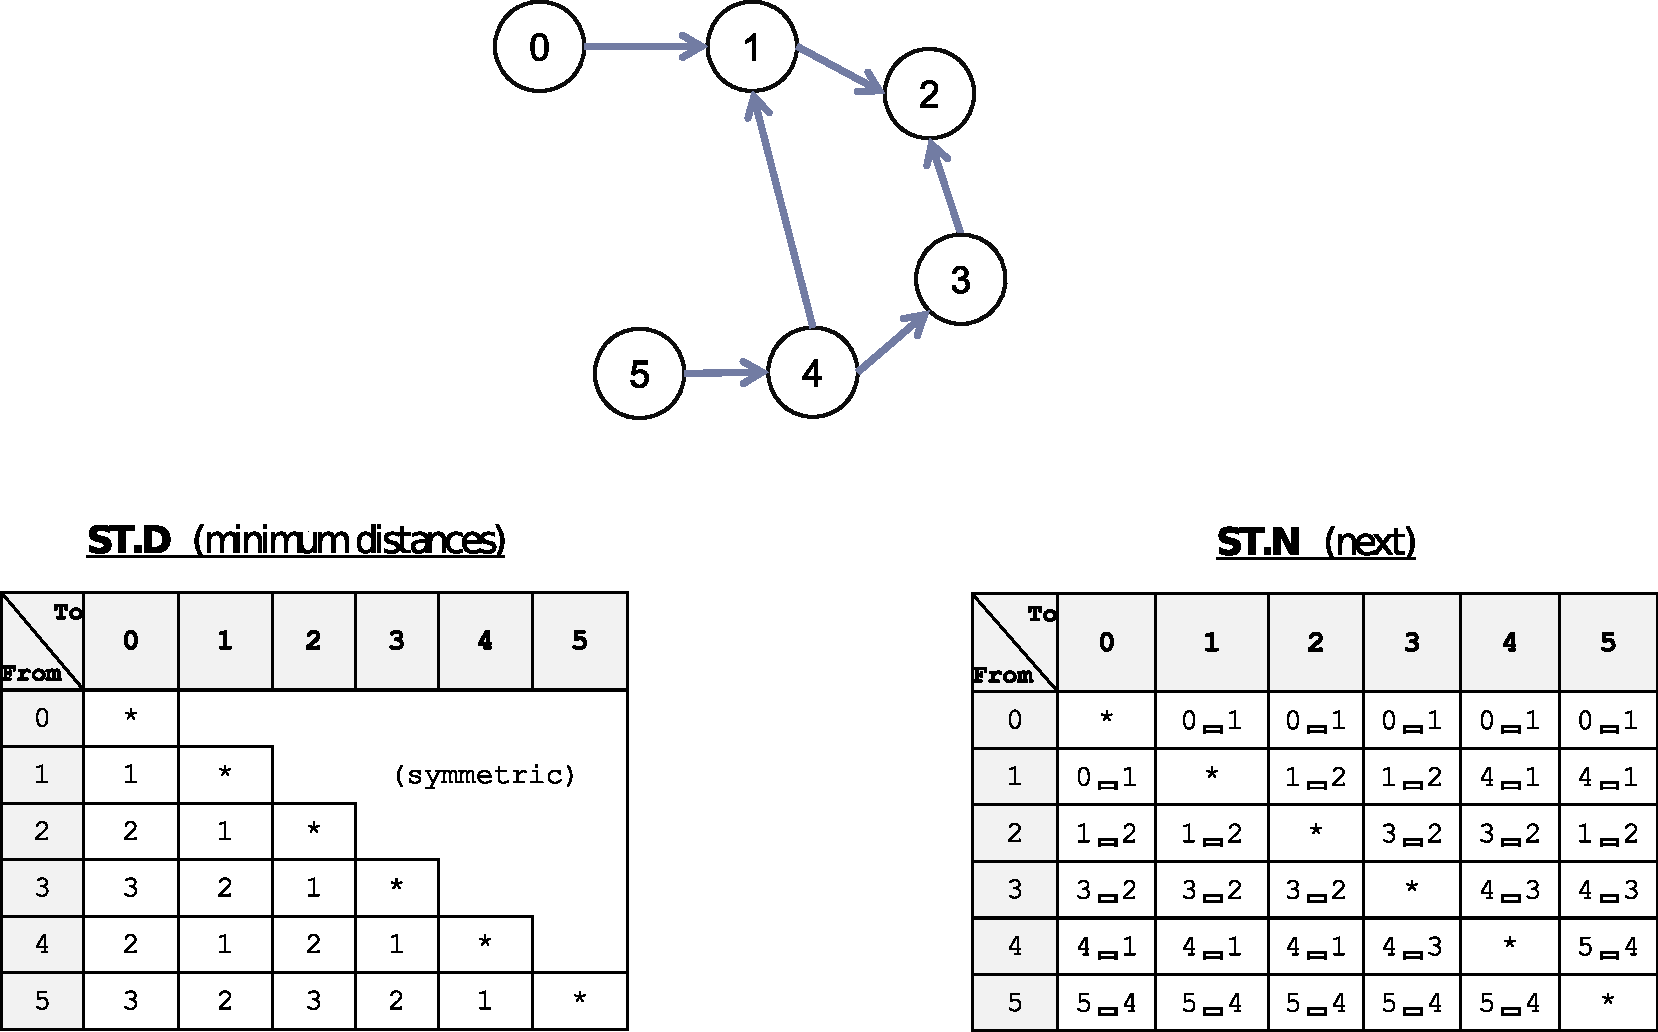
\includegraphics[width=1.0\textwidth]{imgs/spanning-tree-tables.pdf} 
\caption{(top) An example RBA problem. (left-bottom) The $ST.D$ table. (right-bottom) The $ST.N$ table.}
\label{fig:STs2}
\end{figure}

\clearpage

\newpage
\section{Library inner structure}

\subsection{Directory layout}

As said above, \texttt{libmrpt-srba} is a header-only library. 
Thus the headers include both: ``public'' declarations and template implementations. 

The user normally includes just one public header,

\begin{lstlisting}
 #include <mrpt/srba.h>
\end{lstlisting}

\noindent which in turn includes all the other required headers. 
However, thinking of those programmers that intend modifying or extending the library, 
the directory layout of all headers is explained below. 

\begin{itemize}[label=$\rhd$]
  \item{\textbf{mrpt}
    \begin{itemize}[label=$\rhd$]
    \item{\texttt{srba.h}: The main file that users should include.}
    \item{\textbf{srba}
      \begin{itemize}[label=$\rhd$]
      \item{RbaEngine.h}
      \item{(other``public'' headers)}
      \item{\textbf{models}
	\begin{itemize}[label=$\rhd$]
	  \item \texttt{kf2kf\_poses.h}
	  \item \texttt{landmarks.h}
	  \item \texttt{observations.h}
	  \item \texttt{sensors.h}
	\end{itemize}
      }
      \item{\textbf{impl}
	\begin{itemize}[label=$\rhd$]
	\item Implementations of template methods.
	\end{itemize}
	}
      \end{itemize}
    }
    \end{itemize}
  }
\end{itemize}



\subsection{Data structures}
\label{sect:data.structs}

All the data types and containers employed in this library 
have been carefully selected taking into account that the goal
is achieving a constant (bounded) computational cost: no matter 
how many keyframes ($N$) or landmarks ($M$) already exist in the problem, 
introducing a new keyframe with a bounded number of observations
should \emph{never} lead to operations that scale with $N$ or $M$, not even logarithmically.

This need has materialized into the requirement of a network of crossed \emph{references} (in the C++ sense)
between the different containers, which may seem quite complex at first glance but 
is necessary to avoid look-up operations and assure the efficiency of all the SRBA sub-algorithms. 

A detailed view of these relationships is provided in Fig.~\ref{fig:detailed.data.structures} 
for the reference of those interested in the low-level implementation details.

\begin{sidewaysfigure}
\centering
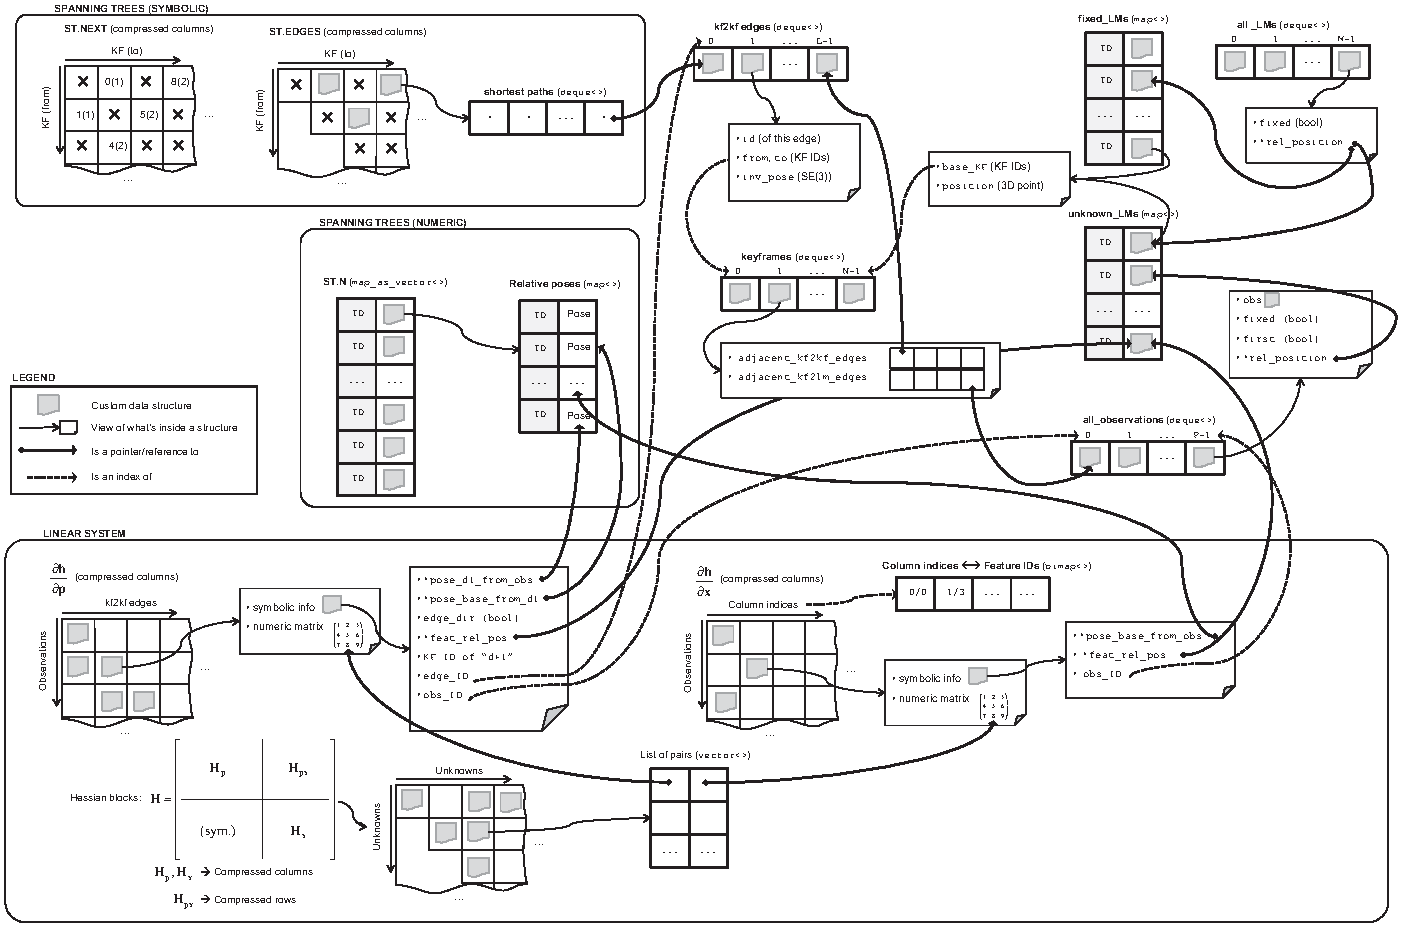
\includegraphics[width=1.0\textwidth]{imgs/srba_data_structures.pdf} 
\caption{Detailed data structures. Refer to the legend for the format of structures and pointers/references.}
\label{fig:detailed.data.structures}
\end{sidewaysfigure}



\newpage
\section{Pseudo-code}

These symbols are employed in the following:

\begin{itemize}
\item{$D_{max}$: Maximum depth for which spanning trees are maintained. It is also the maximum topological distance 
   from the given KF to look for unknowns to optimize during a ``local area'' optimization. Obviously, all KFs within 
   that distance are also in the spanning tree.}
\item{$N_o$: Number of observed landmarks from the new KF being inserted in the problem.}
\item{$N_R$: The maximum number of reachable KFs for a fixed $D_{max}$. It is reasonable to consider that this number 
is bounded for any map, as long as redundant KFs are not continuously added for the same area. 
Figure~\ref{fig:Nr} illustrates the meaning of $N_R$, in a particular example where the local optimization is performed
centered at the keyframe $\#5$.
\begin{figure}[h!]
\centering
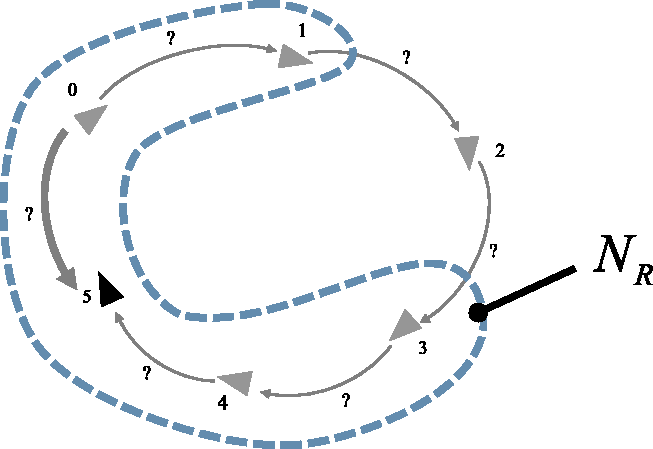
\includegraphics[width=0.5\textwidth]{imgs/Nr.pdf} 
\caption{Example regarding the definition of $N_R$. Here, $N_R=5$ including the origin $\#5$.}
\label{fig:Nr}
\end{figure}
}
\item{$\gamma$: A constant coefficient that models the ``sparseness'' of the graph being solved by least-squares minimization.}
\item{$(\mathbf{z}_n^i,\mathbf{\alpha}_n^i)$: The $i-th$ individual observation of the $n-th$ time step, and 
  its corresponding data association (i.e. its correspondence, the ID of an existing landmark or a new ID if this 
  is a new LM).}
\end{itemize}


\newpage
\subsection{\texttt{define\_new\_keyframe()}}
\label{sect:code:define_new_keyframe}

%% ==============================================
%%  Alg: define_new_keyframe
%% ==============================================
%% ==============================================
%%  Alg: srba_process_new_kf
%% ==============================================
\begin{algorithm}
\BeginAlgSize
\caption{\texttt{srba\_define\_new\_keyframe}   \hfill 
 \textcolor{white}{.}
$\text{Worst case: }\Or( (\gamma N_R)^3+ N_o ( D_{max} + \log N_R)  )$  }
\label{alg:srba}
\begin{algorithmic}[1]
\Statex{C++: \texttt{RBA\_Problem::define\_new\_keyframe()}}
\Statex
  %\medskip
\Require{ $\left( \mathbf{z}_n,\mathbf{\alpha}_n \right) =
\left\{ \left( \mathbf{z}^1_n,\A^1_n \right),...,
   \left( \mathbf{z}^{N_o}_n,\A^{N_o}_n \right) \right\}$ 
\Comment{Set of $N_o$ new observations 
$\mathbf{z}^i_n$ and their data association $\A^i_n$ }}
\Require{ $run\_local\_optimization$ \Comment{Whether to also run optimizations}}
\Ensure { The updated, locally consistent map }
\Statex
%-----------
\Statex{\underline{// Update keyframes (KFs) data structures}}
\State{$n \gets $number of KFs in the map} \Comment{Assign a free ID to the new KF -- $\Or(1)$}
\State{$KF[n] \gets $empty KF data structure} \Comment{Insert at the end of \texttt{std::map} --
$\Or(1)$}
%-----------
\Statex
\Statex{\underline{// Apply edge-creation policy to decide how to handle loop closures, etc.}}
%% \State{$\mathbf{new\_edges} = \varnothing $}
\While{$ \varnothing \neq \left[ (i_k \leftrightarrow n) = \text{\texttt{decide\_edge\_to\_create}()}\right]$ }
  \Comment{\begin{tiny}$\Or(N_o \log N_R)$\end{tiny}}
	\State{\texttt{add\_kf2kf\_edge}$( i_k \leftrightarrow n )$ } 
	\Comment{Update KF-to-KF edge structures -- $\Or(1)$ }
\State{\texttt{update\_sym\_spanning\_trees}$( i_k \leftrightarrow n )$ }
\Comment{$\Or(N_R^2\log N_R)$}
\EndWhile \Comment{Typ. iterations: $\Or(\gamma)$}

%% ---
%-----------
\Statex
\Statex{\underline{// Update symbolic Jacobian structures}}
 \Comment{$\Or\left(N_o (D_{max}+ \log N_R) \right)$}
\ForEach{$ \left( \mathbf{z}_n^i,\mathbf{\alpha}_n^i \right) \in \left(
\mathbf{z}_n,\mathbf{\alpha}_n \right)$}  
\Comment{For each of the $N_o$ new observations}
	\State{\texttt{add\_observation}$(
 \underbrace{\mathbf{z}_n^i}_{\text{obs. data}},
 \underbrace{n}_{\text{observing KF}},
 \underbrace{\mathbf{\alpha}_n^i}_{\text{\text{landmark ID}}} 
)$ }
\Comment{\begin{tiny}$\Or(D_{max}+ \log N_R)$\end{tiny}}
\EndFor
%-----------
\Statex
\If{$run\_local\_optimization$}
\If{$optimize\_new\_edges\_alone$}
\Statex{~~~~~~~~\underline{// Initialize new edges}}
\ForEach{$ (i_k \leftrightarrow n) $} \Comment{For each new kf2kf edge created above}
\State{\texttt{non\_linear\_optimizer}$\left( i_k \leftrightarrow n \right)$} \Comment{$\Or(N_o)$}
\EndFor
\EndIf
%-----------
\Statex
\Statex{~~~~\underline{// Update SLAM estimation}}
\State{$\mathbf{edges\_to\_optimize} \gets$ all within a $D_{max}$ distance from $n$}
\Comment{$\Or(N_R)$}
\State{\texttt{non\_linear\_optimizer}$\left( \mathbf{edges\_to\_optimize}
\right)$} \Comment{$\Or( (\gamma N_R)^3)$}
\EndIf
\end{algorithmic}
\EndAlgSize
\end{algorithm}




\newpage
\subsection{\texttt{update\_sym\_spanning\_trees()}}

This algorithm is explained in \cite{blanco2013srba}.

%% ==============================================
%%  Alg: update_sp_sym
%% ==============================================
%% ==============================================
%%  Alg: update_sp_sym
%% ==============================================
\begin{algorithm}
\BeginAlgSize
\caption{\texttt{update\_sym\_spanning\_trees} \hfill 
 \textcolor{white}{.}
$\text{Worst case: }\Or(N_R^2 \log N_R)$ }
\label{alg:update_sp_sym}
\begin{algorithmic}[1]
  %\medskip
\Require{~\newline 
$(i_k \leftrightarrow n) $ \Comment{A new edge} }\newline
$D_{max}$ \Comment{The maximum desired depth of span. trees}
\Statex
%-----------
  \State{$ST_{D_{max}-1}(i_k) \gets \{ \forall v / d(v,i_k)\leq D_{max}-1 \}$}
    \Comment{$\Or(N_R)$}
  \State{$ST_{D_{max}}(n) \gets \{ \forall v / d(v,n)\leq D_{max} \}$}
    \Comment{$\Or(N_R)$}
   %\Comment{Changes with each $i_k$}
  \Statex
  \ForEach{$r \in ST_{D_{max}}(n)$} \Comment{$\Or(N_R)$ iterations}
   \ForEach{$s \in ST_{D_{max}-1}(i_k)$} \Comment{$\Or(N_R)$ iterations}
    \State{// New tentative distance between $r$ and $s$}
    \State{$d \gets \mathcal{ST.D}[n][r] + \mathcal{ST.D}[i_k][s] + 1 $}
      \Comment{$\Or(\log N_R)$}
     %\Comment{$\Or(\log X)$}
    \If{$\left(s \in \text{\texttt{spanning\_tree}}(r) \text{ \textbf{and} } d < \mathcal{ST.D}[r][s]\right)$ 
$\text{ \textbf{or} }$ $\left(s \notin \text{\texttt{spanning\_tree}}(r) \text{ \textbf{and} } d \leq D_{max}\right)$}
     \Comment{$\Or(\log N_R)$}
       \State{// Shorter or new path found. Update trees:}
       \State{$\mathcal{ST.D}[r][s] \gets d$}
       \State{$\mathcal{ST.N}[r][s] \gets \left\{
	\begin{array}{ll}
	  i_k  & r =n \\
	  \mathcal{ST.N}[r][n] & r \neq n 
	\end{array}
	\right. $}
       \State{$\mathcal{ST.D}[s][r] \gets d$}
        \Comment{$\Or(\log N_R)$}
       \State{$\mathcal{ST.N}[s][r] \gets \left\{
	\begin{array}{ll}
	  n  & s = i_k \\
	  \mathcal{ST.N}[s][i_k] & s\neq i_k 
	\end{array}
	\right. $}
    \EndIf
   \EndFor
  \EndFor
\end{algorithmic}
\EndAlgSize
\end{algorithm}
%% ==============================================






%% ---------------------------------------------------------------
%%                         BIBLIOGRAPHY
%% ---------------------------------------------------------------
\newpage
\bibliographystyle{plain}
\bibliography{cites}

\end{document}

